\documentclass[11pt,a4paper]{article}
\usepackage{graphicx}
\usepackage{amsmath}
\usepackage{listings}
\usepackage{natbib}
\usepackage{graphicx}
\usepackage{amsmath}
\usepackage{listings}
\usepackage{float}

\title{\textbf{ENDSEM 2022: ANTENA CURRENT IN HALF WAVE DIPOLE ANTENA}} % Title

\author{SUHAS C - EE20B132} % Author name
\date{\today}% Date for the report

\begin{document}

\maketitle

\section{Aim :}
\begin{itemize}

\item Obtaining the current using known values like boundary conditions.
\item Finding J  (M-Q)*J=Im*QB equation
\end{itemize}

\newline
\section{Pseudo-code}
\begin{itemize}
\item First run the program and call current function. 
\item Allocate some variable to the given values and find Rz,Ru,P,PB,Q,QB
\itemFind J and current using  (M-Q)*J=Im*QB equation and by initial conditions respectively 
\item Plot currents and compare them.
\end{itemize}

\lstset{language=Python}
\lstset{frame=lines}
\lstset{label={lst:code_direct}}
\lstset{basicstyle=\footnotesize}
\begin{lstlisting}
from pylab import *
import system-function as name
Note: lstsq is found as scipy.linalg.lstsq
ones(List)
zeros(List)
range(N0,N1,Nstep)
arange(N0,N1,Nstep)
linspace(a,b,N)
logspace(log10(a),log10(b),N)
X,Y=meshgrid(x,y)
where(condition)
where(condition & condition)
where(condition | condition)
a=b.copy()
lstsq(A,b) to fit A*x=b
A.max() to find max value of numpy array (similalry min)
A.astype(type) to convert a numpy array to another type (eg int)
def func(args):
...
return List
matrix=c_[vector,vector,...] to create a matrix from vectors
figure(n) to switch to, or start a new figure labelled n
plot(x,y,style,...,lw=...)
semilogx(x,y,style,...,lw=...)
semilogy(x,y,style,...,lw=...)
loglog(x,y,style,...,lw=...)

\end{lstlisting}
\newline

\section{Code}

\subsection{Question 1}
\lstset{language=Python}
\lstset{frame=lines}
\lstset{label={lst:code_direct}}
\lstset{basicstyle=\footnotesize}
\begin{lstlisting}
"""Question 1"""
#Calculating Vector Z 
z = np.linspace(-l,l,2*N+1)

#Calculating u vector
u = np.arange(1, 2*N)
#Removing the middlemost element
u = np.delete(u, N-1, axis=0)

#Calculating the I vector(standard expression ) - the actual I
Current_Vector = np.zeros(2*N+1)
Current_Vector[0:N] = Maximum_Current*sin(k*(l+z[0:N])) # for -l < z < 0
Current_Vector[N:2*N+1] = Maximum_Current*sin(k*(l-z[N:2*N+1])) # for 0 < z < l
I = Current_Vector

#Applying the given Boundary Condition

Unknown_Current=I[u]
\end{lstlisting}

\subsection{Question 2}
\lstset{language=Python}
\lstset{frame=lines}
\lstset{label={lst:code_direct}}
\lstset{basicstyle=\footnotesize}
\begin{lstlisting}

""" QUESTION - 2 """
# Function to compute and return matrix M, H_phi
def H_p(J,n=N,r=a):
	Matrix = (1/(2*pi*r))*(identity(2*N-2))
	V = np.dot(Matrix,J)
	return Matrix,V

Matrix,H_phi = H_p(Unknown_Current,N,a) # Getting the matrix M
\end{lstlisting}

\subsection{Question 3}
\lstset{language=Python}
\lstset{frame=lines}
\lstset{label={lst:code_direct}}
\lstset{basicstyle=\footnotesize}
\begin{lstlisting}
""" QUESTION - 3 """
# Computing vectors Rz, Ru and matrices PB, P
r = a
def Rij(z,r=a):
	ziz,zjz = np.meshgrid(z,z) #Return coordinate Matrices from coordinate vectors
	Radius = sqrt((ziz-zjz)**2 + r**2*np.ones((2*N+1,2*N+1)))
	return Radius

Rz = Rij(z,a)

def Riju(z,u,r=a):
	ziu,zju = np.meshgrid(z[u],z[u]) #Return coordinate Matrices from coordinate vectors
	R = sqrt((ziu-zju)**2 + r**2*np.ones((2*N-2,2*N-2)))
	return R
	
Ru = Riju(z,u,a)

def pij(r,k=k,z=dz):
	P = ((mu0/(4*pi))*(exp(-1j*k*r))*z/r)
	return P
	
P_ij = pij(Ru,k,dz)

RiN = Rz[N]
RiN = np.delete(RiN,[0,N,2*N],0)

Eq_0 = (exp(-1j*k*RiN))

P_B = ((mu0/(4*pi))*(Eq_0)*dz/RiN)

Eq_1 = (-1j*k/Ru)-(1/Ru**2)
Eq_2 = (-1j*k/RiN)-(1/RiN**2)
\end{lstlisting}

\subsection{Question 4}
\lstset{language=Python}
\lstset{frame=lines}
\lstset{label={lst:code_direct}}
\lstset{basicstyle=\footnotesize}
\begin{lstlisting}
""" QUESTION - 4 """
# Computing the matrices Qij and QB

Q_ij = -P_ij*(r/mu0)*(Eq_1)
Q_B = -P_B*(r/mu0)*(Eq_2)
\end{lstlisting}

\subsection{Question 5}
\lstset{language=Python}
\lstset{frame=lines}
\lstset{label={lst:code_direct}}
\lstset{basicstyle=\footnotesize}
\begin{lstlisting}
""" QUESTION - 5 """
# Solving for the current vector, I and comparing with the actual expression
#M1 = identity(2*N-2)/(2*pi*a)

Matrix_1 = np.identity(2*N-2)/(2*pi*r)
Unknown_Current_1 = dot(linalg.inv(Matrix_1-Q_ij),Q_B)

#Printing all the Matrices
print((Rz).round(2))
print((Ru).round(2))
print((P_ij).round(2))
print((P_B).round(2))
print((Q_ij).round(2))
print((Q_B).round(2))

# Finding I(expected value of current)
# Adding the three values given in question

Current_1 = np.insert(Unknown_Current_1,0,0)
Current_1 = np.insert(Current_1,N,Maximum_Current)
Current_1 = np.insert(Current_1,2*N,0)

plt.figure(1)
plt.plot(z,Current_1)
plt.plot(z,I)
plt.grid(True)
plt.savefig("/figure1.png")
plt.show()

print((I).round(2))
print((Current_1).round(2))

\end{lstlisting}
\section{Printing the matrices}
  At N = 4

\newline
\subsection{\item   Matrix Rz:}
\begin{figure}[H]
    \centering
    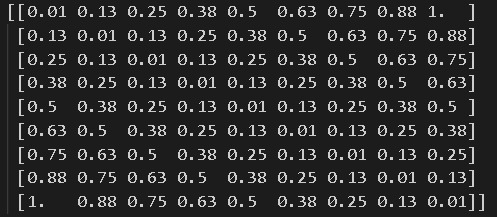
\includegraphics[scale=0.6]{endsem1.jpeg}
    \label{fig:fig}
\end{figure}

\subsection{\item   Matrix Ru:}
\newline
\begin{figure}[H]
    \centering
    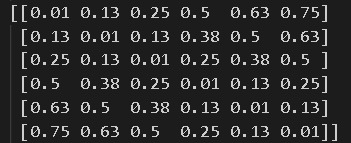
\includegraphics[scale=0.6]{endsem2.jpeg}
    \label{fig:fig}
\end{figure}

\subsection{\item   Matrix P:}
\newline
\begin{figure}[H]
    \centering
    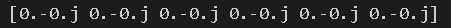
\includegraphics[scale=0.6]{endsem3.jpeg}
    \label{fig:fig}
\end{figure}


\subsection{\item   Matrix PB:}
\newline
\begin{figure}[H]
    \centering
    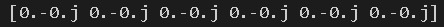
\includegraphics[scale=0.6]{endsem4.jpeg}
    \label{fig:fig}
\end{figure}

\subsection{\item   Matrix Q:}
\newline
\begin{figure}[H]
    \centering
    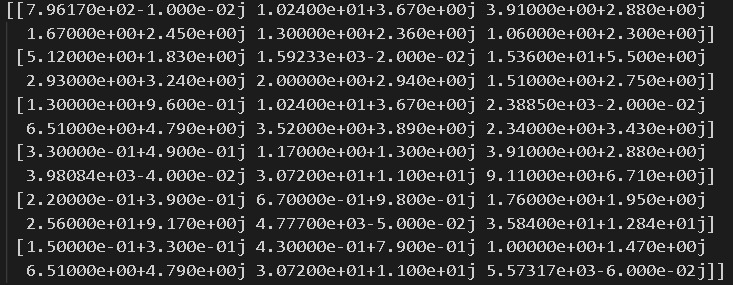
\includegraphics[scale=0.6]{endsem5.jpeg}
    \label{fig:fig}
\end{figure}

\subsection{\item   Matrix QB:}
\newline

\begin{figure}[H]
    \centering
    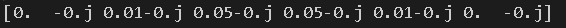
\includegraphics[scale=0.6]{endsem6.jpeg}
    \label{fig:fig}
\end{figure}

\subsection{\item   I assumed:}
\newline
\begin{figure}[H]
    \centering
    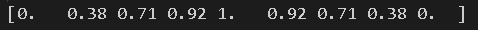
\includegraphics[scale=0.6]{endsem7.jpeg}
    \label{fig:fig}
\end{figure}

\subsection{\item   I derived:}
\newline
\begin{figure}[H]
    \centering
    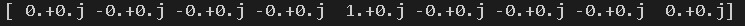
\includegraphics[scale=0.6]{endsem8.jpeg}
    \label{fig:fig}
\end{figure}

\begin{figure}[H]
    \centering
    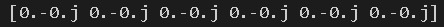
\includegraphics[scale=0.6]{endsem4.jpeg}
    \label{fig:fig}
\end{figure}

\section{plot}
Our final equation is 
\begin{verbatim}
   MJ = QJ +QB
\end{verbatim}
Invert (M-Q) and obtain J. Use inv(M-Q) in python. Add the Boundary currents (zero at i=0, i=2N, and Im at i=N). Then plot this current vs. z and also plot the equation assumed for current at the top of this question paper.
The python code used is as follows
\begin{verbatim}
    J = matmul(inv(Matrix(N, a) - Q) , Q_B) * Im
\end{verbatim}

\subsection{ For N = 100}
\begin{figure}[H]
\centering
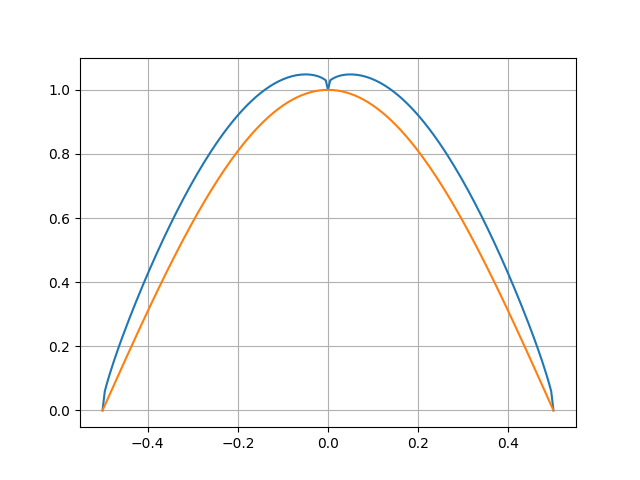
\includegraphics[scale=0.6]{Figure_1.png}
\label{fig:Time domain output of step input}
\end{figure}

\subsection{ For N = 4}
\begin{figure}[H]
\centering
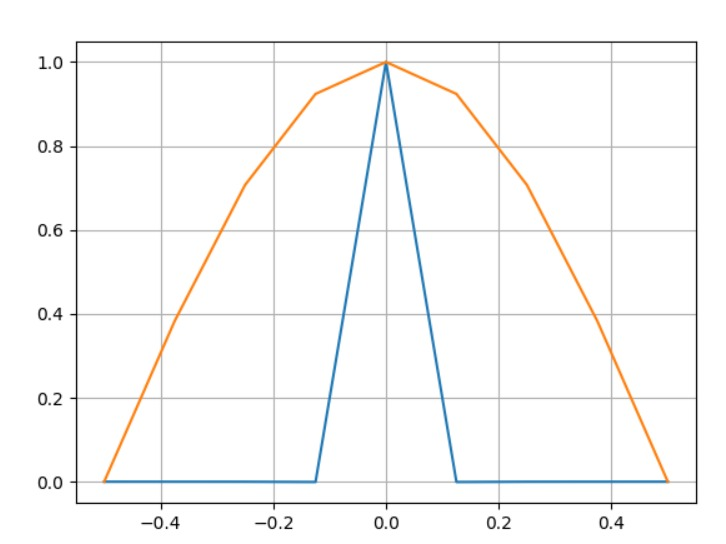
\includegraphics[scale=0.6]{Figure_2.jpeg}
\label{fig:Time domain output of step input}
\end{figure}

\section{Conclusion :}
\begin{itemize}

\item On increasing the value of N,the both graph will merge each other.
\item On increasing N,the magnitude of point which are away from the centre are increasing.
\end{itemize}

\end{document}
